\\
\textbf{Level Structure Overview}\\

Each level is based on an input to output format. Given an initial input, the player
will be expected to use a set of given instructions to manipulate the data to
match an expected output for the puzzle level they are currently on. If their
created output matches the expected output for that level, they have passed the level.
Otherwise, they will need to come up with a new set of instructions (maybe just
slightly altered from the previous solution) to create the exact expected output.
Example levels can be found in Figure \ref{fig:Find_Sum} and Figure \ref{fig:Return_Last}.\\

Import components of this prototype include:
\begin{itemize}
  \item Registers
  \item Input
  \item Output
  \item Instructions
\end{itemize}

\textbf{Registers}\\

The puzzle game will rely on a color-based memory indexing system to access and
manipulate game data. Colors will be used when accessing data structure indices,
although this only applies to registers for now. Two basic blue and red registers
can be seen in Figure \ref{fig:Register_Examples}.

\begin{figure}[!hb]
  \caption{Register Examples}
  \label{fig:Register_Examples}
  \centering
  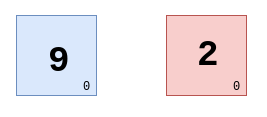
\includegraphics[scale=0.6]{JB_Prototype_Registers.png}
\end{figure}

Consider being shown these two colored boxes. The contents of the box are represented
as the large, centered numbers in bold. The indices of the box are represented as the
small number at the bottom right-hand corner. Indices tell you where to look in a
data structure (redundant for now, since registers only get one index).

\begin{itemize}
  \item Figure \ref{fig:Register_Indexing} shows how to access the 9 in the blue register.
  \begin{itemize}
    \item (called: blue sub 0)
  \end{itemize}
  \item Figure \ref{fig:Register_Indexing} also shows how to access the 2 in the red register.
  \begin{itemize}
    \item (called: red sub 0)
  \end{itemize}
\end{itemize}

\begin{figure}[!hb]
  \caption{Register Indexing}
  \label{fig:Register_Indexing}
  \centering
  
\includegraphics[scale=0.6]{JB_Prototype_Register_Indexing.png}
\end{figure}

From now on, these data structures of size 1, that only contain the index 0, will
be referred to as registers. A specific register and its index is said to be a
memory location.\\

\textbf{Input}\\

Input is data that is given to you initially. This may include one register or
multiple registers, as shown in Figure \ref{fig:Input_Example}.\\

\begin{figure}[!hb]
  \caption{Input Examples}
  \label{fig:Input_Example}
  \centering
  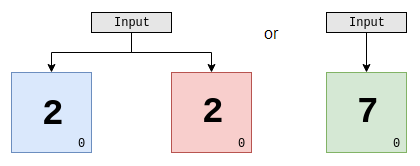
\includegraphics[scale=0.9]{JB_Prototype_Input.png}
\end{figure}

Input can also arrive in the form of an input stream. A stream of input is connected
to one register and continually pushes data from the stream into the register as
data is removed from it (see Figure \ref{fig:Input_Stream}). If there is no more data in the stream,
nothing will be pushed to the register.

\begin{figure}[!hb]
  \caption{Input Stream}
  \label{fig:Input_Stream}
  \centering
  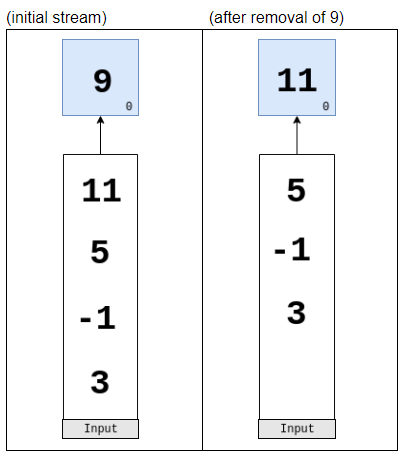
\includegraphics[scale=1]{JB_Prototype_Input_Stream.png}
\end{figure}
\vfill
\clearpage

\textbf{Output}\\

The output is checked at the end of the program. It is up to the player to link
the output to the correct data structure (only registers for now), as well as to
make sure the contents of the data structure match the expected output for the level.
A basic register to output linking can be seen in Figure \ref{fig:Output_Basic}.

\begin{figure}[!hb]
  \caption{Register to Output}
  \label{fig:Output_Basic}
  \centering
  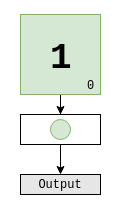
\includegraphics[scale=0.6]{JB_Prototype_Output_Basic.png}
\end{figure}

The green circle specifies that the contents of the green data structure will be
returned as the output for the player's solution to the puzzle level.\\

Consider a scenario in which multiple data structures may be returned as output.
In the following example (Figure \ref{fig:Output_Choice}), the player needs to return the register
with the greater value by choosing which colored data structure to link to the output.

\begin{figure}[!hb]
  \caption{Output Choice}
  \label{fig:Output_Choice}
  \centering
  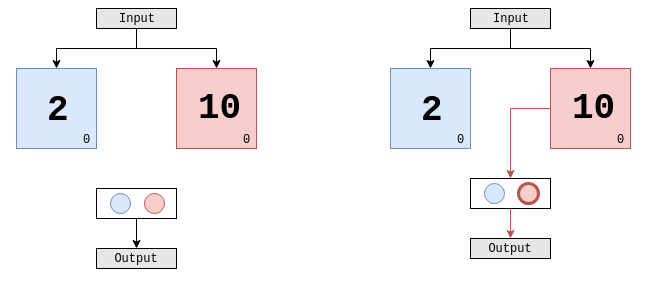
\includegraphics[scale=0.7]{JB_Prototype_Output_Choice.png}
\end{figure}

Players can link data structures to output by simply choosing the corresponding colored
circle of the data structure they would like to return. Clearly 10 is greater than 2 here and
the red register should returned.\\

\textbf{Instructions}\\

The notable instructions are as follows:

\begin{itemize}
  \item Move
  \item Return
  \item Add
  \item Subtract
  \item Jump
\end{itemize}

Instructions are clicked or dragged from a limited set of given instructions, 
specific to each level.\\

When the player is ready to test their solution, each instruction will execute
procedurally from top to bottom.\\

It is up to us to structure the levels and instructions given in each level in such
a way that minimizes the amount of errors the player can create. Runtime errors
are okay, but we should strive to avoid having the player feel as if they are learning
syntax. We would also like to avoid confusing the player by giving a limited
instruction set for each level with thorough explanations for each instruction.\\

Parameters used in certain instructions (Move, Return, Add, Subtract) are chosen
from a drop down menu, again minimizing the amount of errors the player can create
on their own. When choosing a colored data structure and an index, only the colors of
the data structures and their valid indices that are already on the puzzle board
are given as options in the drop down menu.\\
\newpage

\textbf{Instruction: Move}\\

The move instruction takes two arguments, a source register and a destination register.
It's main functionality consists of three different parts:

\begin{itemize}
  \item Move the contents of the source to the destination
  \item Leave the contents of the source unchanged
  \item Override the previous contents of the destination
\end{itemize}

How the instruction would look in the instruction editor is shown in Figure
\ref{fig:Move_Instruction}.

\begin{figure}[!hb]
  \caption{Move Instruction}
  \label{fig:Move_Instruction}
  \centering
  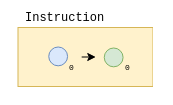
\includegraphics[scale=1]{JB_Prototype_Move.png}
\end{figure}

The contents of the two registers before and after the move instruction is
received is shown in Figure \ref{fig:Move_Instruction_Use}.

\begin{figure}[!hb]
  \caption{Move Instruction In Use}
  \label{fig:Move_Instruction_Use}
  \centering
  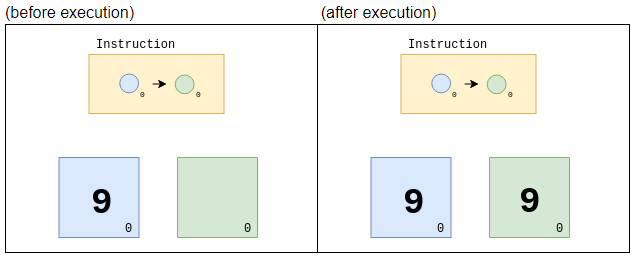
\includegraphics[scale=0.8]{JB_Prototype_Move_Use.png}
\end{figure}

Each argument (left and right side of the arrow) will have two drop down menus:
\begin{itemize}
  \item Color of register
  \item Index of register
\end{itemize}

The move instruction is atomic and meant to abstract the process of manually
picking up the data and placing it down.\\

\textbf{Instruction: Return}\\

The return instruction will specify only one argument -- which colored data structure
to return as output.
\begin{itemize}
  \item A return instruction is required for every level
  \item May be given, or may require the player to write it
  \item The data structure that is returned is compared against the expected
  output for the level
\end{itemize}

Figure \ref{fig:Return_Instruction} shows how the return instruction looks in the instruction editor.

\begin{figure}[!hb]
  \caption{Return Instruction}
  \label{fig:Return_Instruction}
  \centering
  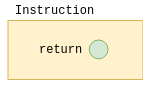
\includegraphics[scale=0.8]{JB_Prototype_Return.png}
\end{figure}

The argument is chosen from a drop down menu that allows the player to select
the color of the data structure they want to return.\\

Using the example from the output section (Figure \ref{fig:Output_Choice}),
we can show the correct usage of the return instruction in Figure \ref{fig:Return_Instruction_Use}.

\begin{figure}[!hb]
  \caption{Return Instruction In Use}
  \label{fig:Return_Instruction_Use}
  \centering
  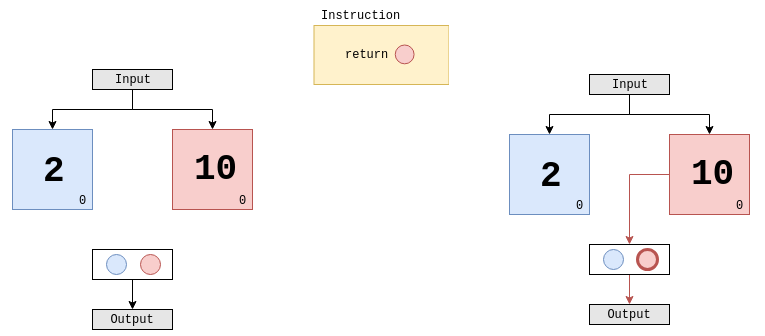
\includegraphics[scale=0.7]{JB_Prototype_Return_Use.png}
\end{figure}
\vfill
\clearpage

\textbf{Instruction: Add}\\

The add instruction takes three arguments:
\begin{itemize}
  \item Two memory locations to be added
  \item The destination of their sum, another memory location
\end{itemize}

Figure \ref{fig:Add_Instruction} shows how the add instruction looks in the
instruction editor.

\begin{figure}[!hb]
  \caption{Add Instruction}
  \label{fig:Add_Instruction}
  \centering
  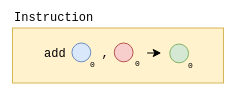
\includegraphics[scale=0.8]{JB_Prototype_Add.png}
\end{figure}

When referencing the memory locations, an index must also be specified, as we've
seen before. Figure \ref{fig:Add_Instruction_Use} shows the add instruction in use by displaying
the contents of the registers included in the instruction before and after it is
run.

\begin{figure}[!hb]
  \caption{Add Instruction In Use}
  \label{fig:Add_Instruction_Use}
  \centering
  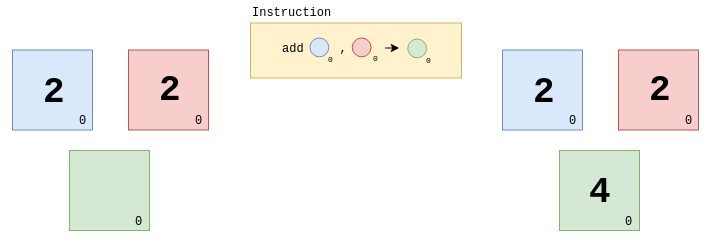
\includegraphics[scale=0.7]{JB_Prototype_Add_Use.png}
\end{figure}

Note:\\
The destination can be one of the source registers used, in which case it would
just overwrite the data, similarly to how the move instruction functions.\\
\newpage

\textbf{Instruction: Subtract}\\

The subtract instruction works exactly the same as the add instruction above,
although the difference of the two registers is placed into the destination, rather
than the sum.\\

Figure \ref{fig:Sub_Instruction} shows how the subtract instruction looks in the
instruction editor.

\begin{figure}[!hb]
  \caption{Subtract Instruction}
  \label{fig:Sub_Instruction}
  \centering
  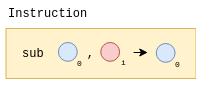
\includegraphics[scale=0.9]{JB_Prototype_Sub.png}
\end{figure}

\textbf{Instruction: Jump}\\

The jump instruction is paired with an anchor. When a jump instruction is executed,
the flow of control immediately jumps to the instruction that lays at the anchor.\\

It is up to the user to choose where the anchor will lie after placing a Jump instruction
in the instruction editor.\\

Figure \ref{fig:Jump_Instruction} shows how the jump instruction looks in the
instruction editor.

\begin{figure}[!hb]
  \caption{Jump Instruction}
  \label{fig:Jump_Instruction}
  \centering
  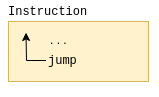
\includegraphics[scale=0.9]{JB_Prototype_Jump.png}
\end{figure}

Figure \ref{fig:Jump_Instruction_Use} shows how the control flow is handled when a jump instruction is
executed.

\begin{figure}[!hb]
  \caption{Jump Instruction In Use}
  \label{fig:Jump_Instruction_Use}
  \centering
  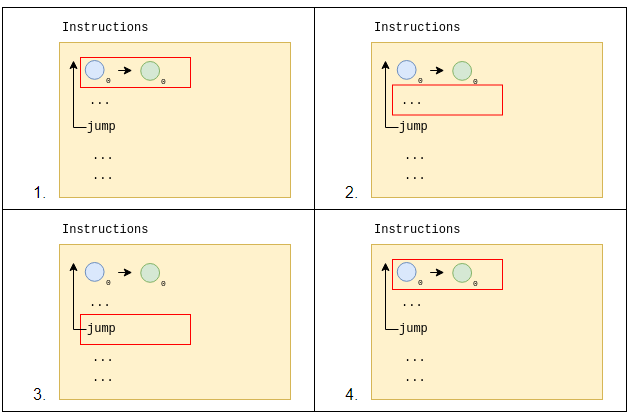
\includegraphics[scale=0.9]{JB_Prototype_Jump_Use.png}
\end{figure}
\vfill
\clearpage

\begin{figure}[!hb]
  \caption{Example Level: Find Sum}
  \label{fig:Find_Sum}
  \centering
  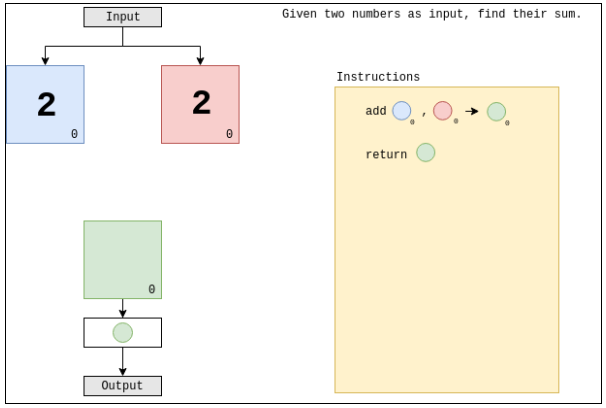
\includegraphics[scale=1]{JB_Prototype_Find_Sum.png}
\end{figure}
\vfill
\clearpage

\begin{figure}[!hb]
  \caption{Example Level: Return Last}
  \label{fig:Return_Last}
  \centering
  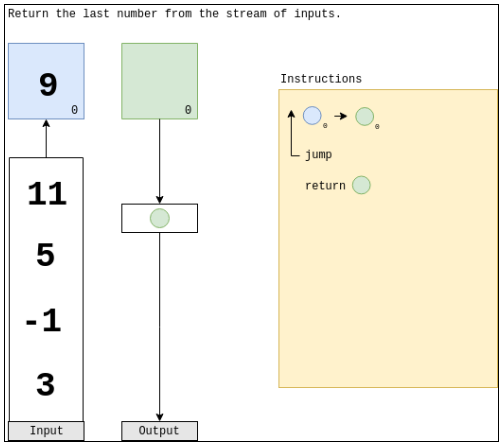
\includegraphics[scale=1]{JB_Prototype_Return_Last.png}
\end{figure}
\vfill
\clearpage

\newpage
